% Lecture 05 How to write the SRS Sep 2021 Complete: https://docs.google.com/document/d/1fnwYnqAYdEQx13KpmQvulktGNpjKAKfx/edit
% Lecture 05 MSc Project - How to write the SRS Chapter: https://docs.google.com/document/d/1lEheSmKF9sDZkRozLTLSJ8XBDC_4yDxL/edit

% 2. We critically evaluated the Chapter 4 of the sample thesis - https://drive.google.com/drive/folders/1GlPK41lsmaZ26HIwK64AFwvb-3u0Chpx?usp=sharing (Visit Chapter 04 of the thesis and see my comments to see how you can improve)

% --------------

\section{Chapter Overview}
This chapter focuses on identifying possible stakeholders of the project by taking a look at all possible points of interaction with the system with the use of a rich picture diagram, gathering their perceptions to analyse and come up with possible expected use cases, functional and non-functional requirements of the prototype. 

\section{Rich Picture}

% rich picture in canva: https://www.canva.com/design/DAEwtvMqut8/k-BGnDBlelk824WGuNdb7g/edit

\begin{figure}[h!]
\centering
\frame{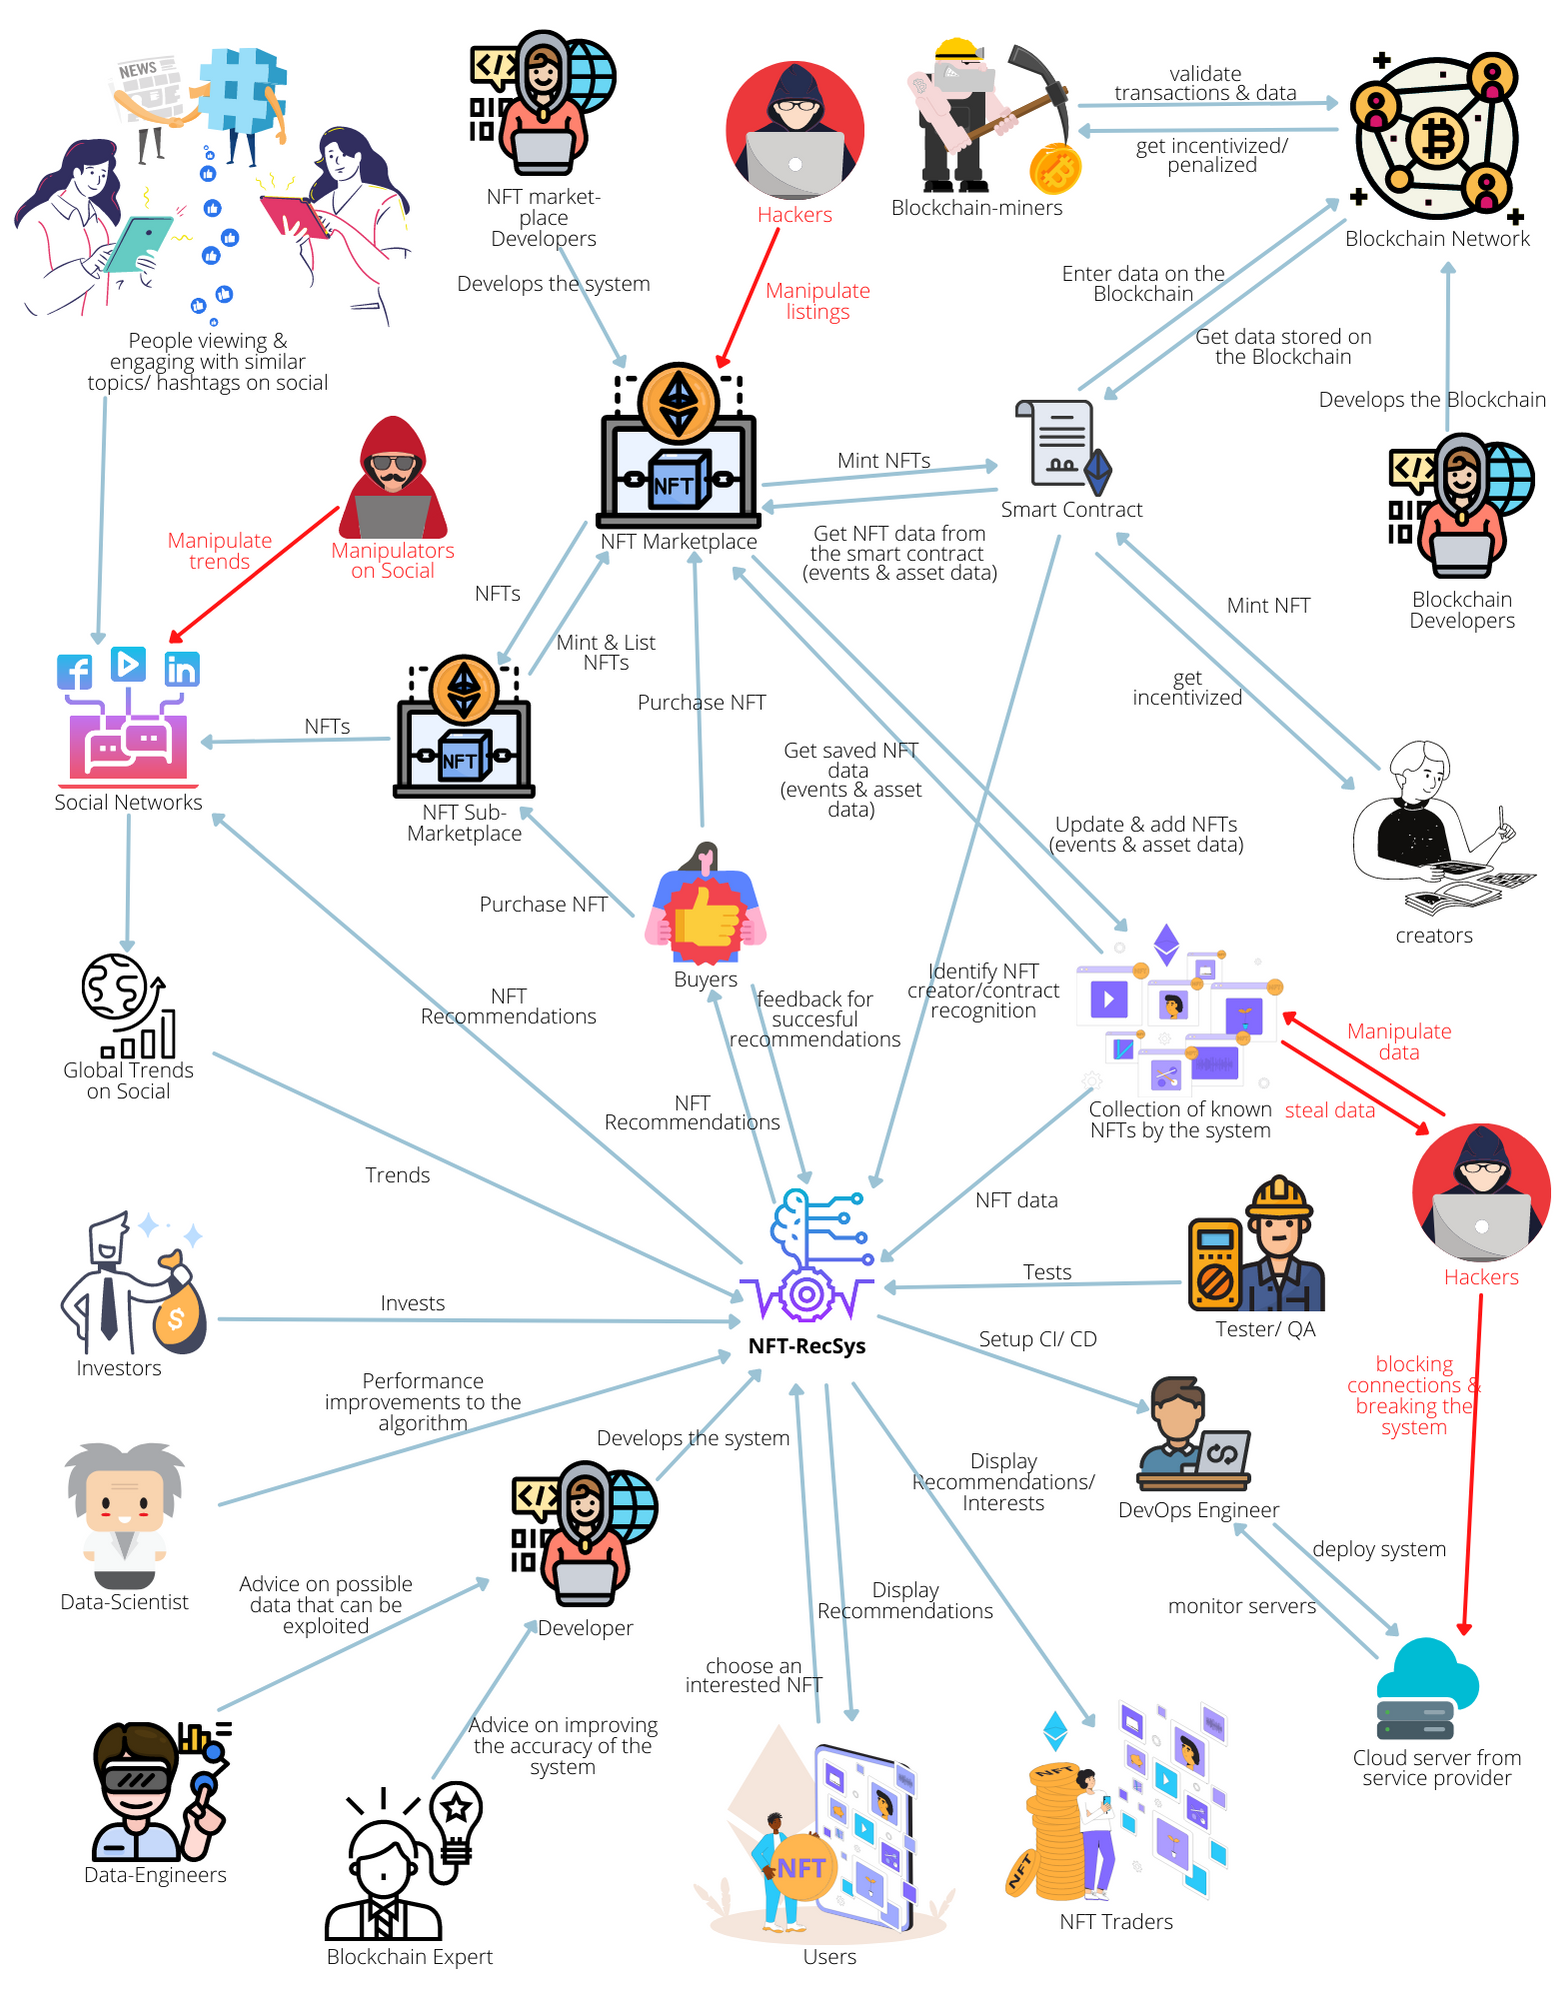
\includegraphics[height=0.65\textheight]{images/SRS/rich-picture.png}}
\caption{Rich Picture Diagram \textit{(self-composed)}}
\label{fig:rich-picture}
\end{figure}

The above Rich Picture diagram shows a helicopter view of how related parties in the rest of the world interacts with the system. It is used to understand the possible interactions that are expected to happen when the system is functional.

\section{Stakeholder Analysis}
The Stakeholder Onion Model illustrates recognized stakeholders who are associated with the system, along with an explanation of each stakeholder's involvement in the system, in Stakeholder Viewpoints.

\subsection{Stakeholder Onion Model}
% figma diagram: https://www.figma.com/file/jEF3LQTiRNXY5tJo6faSDy/FYP---NFT-Recommendation-System?node-id=304%3A3
\begin{figure}[h!]
\centering
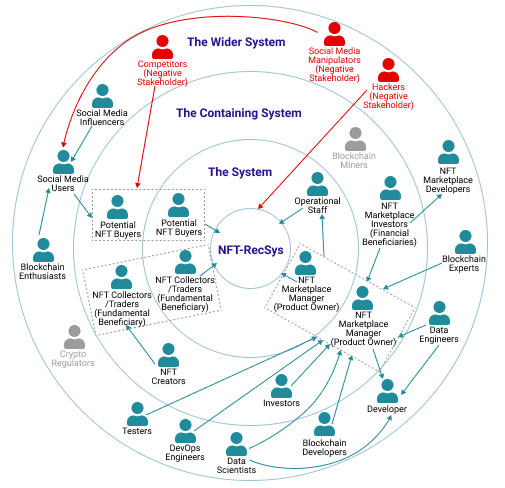
\includegraphics[width=\textwidth]{images/SRS/stakeholder-onion-diagram.png}
\caption{Stakeholder Onion Model \textit{(self-composed)}}
\label{fig:stakeholder-onion}
\end{figure}

\pagebreak
\subsection{Stakeholder Viewpoints}

\vspace{-4mm}       % remove line spacing after

\begin{longtable}{|p{0.2\linewidth}|p{0.23\linewidth}|p{0.51\linewidth}|} 
\caption{Roles and benefits of identified stakeholders}\\ 
\hline
\textbf{Stakeholder} & \textbf{Role} & \textbf{Benefits/ Role Description} \\* 
\hline
Developer & \multirow{2}{*}{Financial Beneficiary} & Develops the system \\* 
\cline{1-1}\cline{3-3}
Investors &  & Makes a profit out of the investments put into marketing, deployments and development of the system \endfirsthead 
\hline
NFT Marketplace Developers & Operational - Maintenance & Integrates the system into NFT Marketplaces. \\* 
\hline
Blockchain Experts & \multirow{3}{*}{\parbox{8em}{Expert, Quality Regulator}} & Provides expert advice \& insights into domain knowledge, to improve the system’s performance. \\* 
\cline{1-1}\cline{3-3}
Data Scientists &  & Provides performance improvements for the performance of the Data scienc models/ algorithms used. \\* 
\cline{1-1}\cline{3-3}
Data Engineers &  & Provides advice on possible data that can be exploited, to make the best possible recommendations. \\ 
\hline
NFT Creators & Financial Beneficiary & Gets a better opportunity to get their creations in the eye of potential buyers. Makes a profit by selling creations to people who are interested in the creations. \\* 
\hline
NFT Traders/ Collectors & \multirow{2}{*}{\parbox{8em}{Fundamental Beneficiary}} & It becomes easier for traders to sell NFTs as well as explore more NFTs to purchase. It also allows them to explore NFTs that may be worth collecting for a future trade. \\* 
\cline{1-1}\cline{3-3}
Potential NFT Buyers &  & It becomes more convenient for these parties to explore NFTs that they’re interested in. \\ 
\hline
NFT Marketplace Manager & System Owner, Operational - Administration & Inputs data sources for opinion mining, sets default biases. Makes sure that the system is up \& running, while managing the operational staff. \\ 
\hline
Operational Staff & Operational - Support & Makes sure that the system is up \& running, while attending to users’ requests \& issues. \\* 
\hline
DevOps Engineers & Product Deployment \& Maintenance & Deploys the system to the cloud and make sure that it’s up \& serving users, without throttling. \\* 
\hline
Social Media Influencers & Operational - Secondary & Influences users on social media and drives trends. \\* 
\hline
Social Media Users & Operational - Secondary \& Fundamental Beneficiary & Get influenced to search for items of interest and possibly turn into potential NFT buyers. \\* 
\hline
Hackers & \multirow{3}{*}{Negative Stakeholder} & May manipulate listings in NFT market places. \\* 
\cline{1-1}\cline{3-3}
Competitors &  & May build competing products that outperform/ undercut pricing. \\* 
\cline{1-1}\cline{3-3}
Social Media Manipulators &  & May manipulate users on social media \& drive trends that a majority of users aren’t interested in. \\ 
\hline
Blockchain Enthusiasts & Operational & Helps drive awareness and keep the public up to date with the latest releases \& feature updates. \\ 
\hline
Blockchain Miners & Operational - Secondary & Helps keep Blockchains up \& running by validating the data on the network. \\ 
\hline
Crypto Regulators & Quality Regulator & May have an impact as a regulator, if the system is used by mainstream networks.\\
\hline
Testers & Quality Inspector & Tests the system \& ensures that it's suitable to run in production.\\
\hline
\end{longtable}


\section{Requirement Elicitation Methodologies}
In order to gather requirements for the development of the research project, there were multiple requirement elicitation methodologies that were followed. literature review, interviews, survey \& prototyping were the methodologies chosen for this purpose.
The reasons to choosing the specified requirement elicitation methodologies have been discussed below.
% Tell why you chose the specified requirement elicitation methodologies

\pagebreak
% \vspace{-4mm}       % remove line spacing after

\begin{longtable}{|p{0.96\linewidth}|}
\caption{Requirement Elicitation Methodologies}\\
\hline
\textbf{Method 1: Literature Review} \\
\hline
At the inception of the project, the author has done a thorough literature review to identify research gaps that are open in the desired field of study and a chosen domain of interest. In order to understand research gaps available in technologies that can be applied, existing systems were studied together with relatable technologies that are possible to be applied to the existing systems that were mentioned in literature. \\
\hline
\textbf{Method 2: Interviews} \\
\hline
Interviews were conducted as a means of gathering expert-insights into domain-specific requirements and also to identify the best possible way to solve the problem at hand while contributing to the body of knowledge through research. 
% When approaching experts to conduct interviews, domain experts were presented with a separate set of questions compared to those presented to technical experts since the
Due to the domain being new and the required technical knowledge being specific, interviews were identified to be the best-possible source of knowledge to gather requirements that align with the research gap. This method also allowed to get qualitative feedback on the proposed system making it possible to identify any drawbacks/ challengers that may have to be addressed while prototyping.
\\
\hline
\textbf{Method 3: Survey} \\
\hline
As a means of conducting a survey, questionnaire was used as a tool to gather requirements and insights from potential users of the proposed system. This form of survey will aid the author in comprehending people's cognitive processes and the expectations they have for the prototype. It will also allow the author to clarify if the proposed solution would be helpful to intended users.\\
\hline
\textbf{Method 4: Prototyping} \\
\hline
Since the project was chosen to follow the \textit{Agile} Software Development Life-cycle, prototyping would allow the author to recursively try out various alternative implementations to identify any areas of improvement while testing and evaluating the prototype.\\
\hline
\end{longtable}

\section{Analysis of Data \& Presentation of the Outcome through Elicitation Methodologies}
The analysis of data gathered through the chosen means of requirement elicitation have been presented below.
% Discuss findings

\pagebreak

\subsection{Literature Review}

\vspace{-4mm}       % remove line spacing after

\begin{longtable}{|p{0.77\linewidth}|p{0.17\linewidth}|} 
\caption{Findings through Literature Review}
\label{tab:lr-findings-table}\\
\hline
\textbf{Finding} & \textbf{Citation} \\ 
\hline
In completion of the review of literature, it was identified that a Recommendations System for \gls{nft}s would benefit the majority of users to make purchase decisions as well as allow them to explore relevant items, that would in return benefit the market places, creators \& traders who are selling them as Recommendations Systems have proven to improve sales of e-commerce sites in the past. & \autocite{naumov_deep_2019, vanderbilt_science_nodate} \\ 
\hline
When exploring technologies that can be applied to achieve the required outcome, it was understood that the use of Deep learning hasn’t been able to improve the output of recommendations compared to other fields of applications, in most cases. & \autocite{choi_local_2021} \\
\hline
It was identified that implementing a custom hybrid ensembled model with the injection of social media trends has not been explored in literature. & \autocite{ayushi_cross-domain_2018, cheng_hybrid_2020} \\
\hline
The use of data from similar users’ timelines for recommendations has been mentioned as possible future work. & \autocite{chen_user_2019} \\
\hline
Pricing of \gls{nft}s \& contract recognition data have not been considered for any previous implementations of Recommender Systems & \autocite{noauthor_what_2020} \\
\hline
The only study related to recommending \gls{nft}s only recommends \gls{nft} collections that a user may be interested in, but not actual \gls{nft}s themselves. & \autocite{noauthor_what_2020} \\
\hline
\end{longtable}


% \begin{longtable}{|p{0.96\linewidth}|}
% \caption{Findings through Literature Review}\\
% \hline
% \textbf{Findings} \\
% \hline
% In completion of the review of literature, it was identified that a Recommendations System for \gls{nft}s would benefit the majority of users to make purchase decisions as well as allow them to explore relevant items, that would in return benefit the market places, creators \& traders who are selling them as Recommendations Systems have proven to improve sales of e-commerce sites in the past.
% \bigbreak
% When exploring technologies that can be applied to achieve the required outcome, it was understood that the use of Deep learning hasn't been able to improve the output of recommendations compared to other fields of applications, in most cases. It was identified that implementing a custom hybrid ensembled model with the integration of social media trends has not been explored in literature. But, the use of data from similar users' timelines has been mentioned as possible future work. Neverthless, it was also identified that pricing of \gls{nft}s \& contract data have not been considered for any previous implementations either. The only study related to recommending \gls{nft}s only recommends \gls{nft} collections that a user may be interested in, but not actual \gls{nft}s themselves.
% \\
% \hline
% \end{longtable}

\subsection{Interviews}
% interview Google form: https://forms.gle/9SchzfH3AzpLVbRo7
% This table can be moved to appendix later, if there's not enough space - have thematic analysis would be enough here.

In order to get opinions of technical as well as domain expertise, interviews were conducted with experts from the respective fields. Experts \& researchers in \gls{ml}, Recommendation Systems and Blockchain were chosen to be interviewed in order to establish project requirements. 3 Blockchain experts, 1 NFT Creator, 1 Senior Data Engineer, 2 PhD students in \gls{ml} and a Data science engineer were interviewed.
% The appendix shall contain more information about the interviewees.
The outcome of interviews were processed to a \textbf{thematic analysis} based on the following themes.


% \begin{longtable}{|p{0.2\linewidth}|p{0.74\linewidth}|}
% \caption{Analysis of feedback from interviews}\\
% \hline
% \textbf{Question} & \textbf{What are the possible factors that a buyer would consider when searching to buy an NFT?} \endfirsthead
% \hline
% \textbf{Aim of question} & To understand the factors to be considered when making a recommendation by the Recommendations System \\
% \hline
% \multicolumn{2}{|l|}{\textbf{Findings}} \\
% \hline
% \multicolumn{2}{|l|}{} \\ 
% \hline
% \textbf{Question} & \textbf{What functionalities would you like to have in a Trading Recommendations System for Non-fungible Tokens?} \\
% \hline
% \textbf{Aim of question} & To identify the non-function requirements of the system, that would make the system as user-friendly as possible \\
% \hline
% \multicolumn{2}{|l|}{\textbf{Findings}} \\
% \hline
% \multicolumn{2}{|l|}{} \\ 
% \hline
% \textbf{Question} & \textbf{Who do you think will be benefited from using this system?} \\
% \hline
% \textbf{Aim of question} & To identify the beneficiaries of the proposed system. \\
% \hline
% \multicolumn{2}{|l|}{\textbf{Findings}} \\
% \hline
% \multicolumn{2}{|l|}{} \\ 
% \hline
% \textbf{Question} & \textbf{Do you think that this system would benefit people who have no expertise in Blockchain/ NFTs as well as people who have a decent amount of expertise in Blockchain/ NFTs?} \\
% \hline
% \textbf{Aim of question} &  To identify how valuable the system would be to people of all levels of expertise in Blockchain/ NFTs \\
% \hline
% \multicolumn{2}{|l|}{\textbf{Findings}} \\
% \hline
% \multicolumn{2}{|l|}{} \\ 
% \hline
% \textbf{Question} & \textbf{How much would you expect a Recommendations System that considers social media trends to be beneficial for businesses to integrate into their online platforms?} \\
% \hline
% \textbf{Aim of question} & To identify the importance of the technological contribution in the project \\
% \hline
% \multicolumn{2}{|l|}{\textbf{Findings}} \\
% \hline
% \multicolumn{2}{|l|}{} \\ 
% \hline
% \textbf{Question} & \textbf{Do you think that a user would benefit more if one platform provides recommendations that differ from another platform with the same dataset?} \\
% \hline
% \textbf{Aim of question} & To identify if the proposed Recommendations System will benefit from implementing a Reinforcement Learning technique to adapt and suite different platforms. \\
% \hline
% \multicolumn{2}{|l|}{\textbf{Findings}} \\
% \hline
% \multicolumn{2}{|l|}{} \\ 
% \hline
% \textbf{Question} & \textbf{Which of the following roles describes your relevance of expertise to this project?} \\
% \hline
% \textbf{Aim of question} & To identify the background of the target audience and identify which of their responses will be more valuable for the domain contribution and technological contribution. \\
% \hline
% \multicolumn{2}{|l|}{\textbf{Findings}} \\
% \hline
% \multicolumn{2}{|l|}{} \\ 
% \hline
% \end{longtable}

% \pagebreak
% \subsubsection{Thematic Analysis of findings from Interviews}

\begin{longtable}{|p{0.22\linewidth}|p{0.72\linewidth}|}
\caption{Thematic analysis of interview findings}\\ 
\hline
\textbf{Theme} & \textbf{Analysis} \endfirsthead 
\hline
Collection \& pre-processing of available data. & As this is expected to be a Data science project, the main concern that all participants had was the availability of data. Clustering of available data was suggested to identify possible patterns by \gls{ml} experts, while Blockchain experts suggested the use of publicly available data on the Blockchain such as details from Smart-Contracts to be used to improve the quality of recommendations. \\ 
\hline
Applicable Recommendation Techniques & The opinion of majority of the interviewees was that this project would benefit more by the use of rule-based algorithmic recommendation models instead of \gls{dl} models due to the constraint of . According to technical experts, having a specialized recommendation model built using algorithms is very highly accepted in industrial applications. They seem to perform better in most new domains according to PhD researches. Even some of the biggest e-commerce organizations in the world seem to benefit a lot by custom-built recommendations algorithms tailored to specified use-cases according to research \& development experts in Recommendation Systems. \\ 
\hline
Integration of Opinion Mining into Recommendation Systems & Domain experts thought that integrating trends and other social opinion will add value to the recommendations. They were also interested in identifying a possibility of checking for the sentiment represented by the opinions as well. When considering social sentiment, Tweets/ opinions of well-known influencers may play a bigger effect into the value of curtain \gls{nft}s. \\ 
\hline
Research gap \& scope &  The technological experts thought that the method that the author proposed was very innovative and that according to their knowledge, they haven't seen a similar integration to the suggested architecture in previous applications. \\ 
\hline
Creating the bias for a Hybrid Recommendations Model & While some of the interviewees suggested the use of a fixed weighted bias, others suggested a variable bias. The method applicable for variable bias or the best-possible fixed bias can be tested via continuous prototyping \& evaluation. The use of user-input was also suggested to identify a possible expected bias.\\ 
\hline
Prototype features \& suggestions & The Data science experts were very interested in seeing a Recommendations System built purely using custom algorithms with the help of vectorization functions that many \gls{ml} libraries support. The use of transfer learning or pre-trained models were suggested for \gls{nlp} parts of the implementation.\\ 
\hline
Understanding a buyer's decision making for automation & The value proposition was identified to be created by an external entity based on contract \& token Ids stored on the blockchain. Due to the difference in real world trust and blockchain trust, this may have to be inferred from the available data such as past contract data and social sentiment from trends. \\ 
\hline
The necessity of NFT-RecSys \& contributions & As the first research study related to a Recommendations System for \gls{nft}s, the interviewees thought that the contribution to the domain will be of great value and also, since the hybrid architecture of the proposed system is novel, the contribution to the technological domain would help the advancement of the quality of recommendations in future implementations. It was also understood that it's difficult to find specific \gls{nft}s based on tags/ characteristics.
% \bigbreak
Furthermore, it was revealed that Sri Lanka does not have Machine Intelligence/ Data science driven Recommendation Systems in all local e-commerce stores.
\\ 
\hline

%  Reinforcement Learning in Recommendation Systems &  \\
% \hline
% Personalized Recommendation Systems &  \\ 
% \hline
\end{longtable}

\pagebreak
\subsection{Survey}
% interview & questionnaire questions: https://docs.google.com/document/d/1oNKIeRZbnVcRPimWl0f07go6Uovjzdk5vwATmVQCbFQ/edit
% survey Google form: https://forms.gle/w2zNTNBjiqZ3KNSg8

\vspace{-4mm}       % remove line spacing after
\begin{longtable}{|p{0.18\linewidth}|p{0.74\linewidth}|}
\caption{Analysis of replies to questionnaire}\\
\hline
\textbf{Question} & \textbf{How will you decide which NFT to purchase?} \endfirsthead
\hline
\textbf{Aim of question} & To understand how a potential buyer would proceed to purchase an NFT. \\
\hline
\multicolumn{2}{|l|}{\textbf{Findings \& Conclusion}} \\

\multicolumn{2}{|l|}{
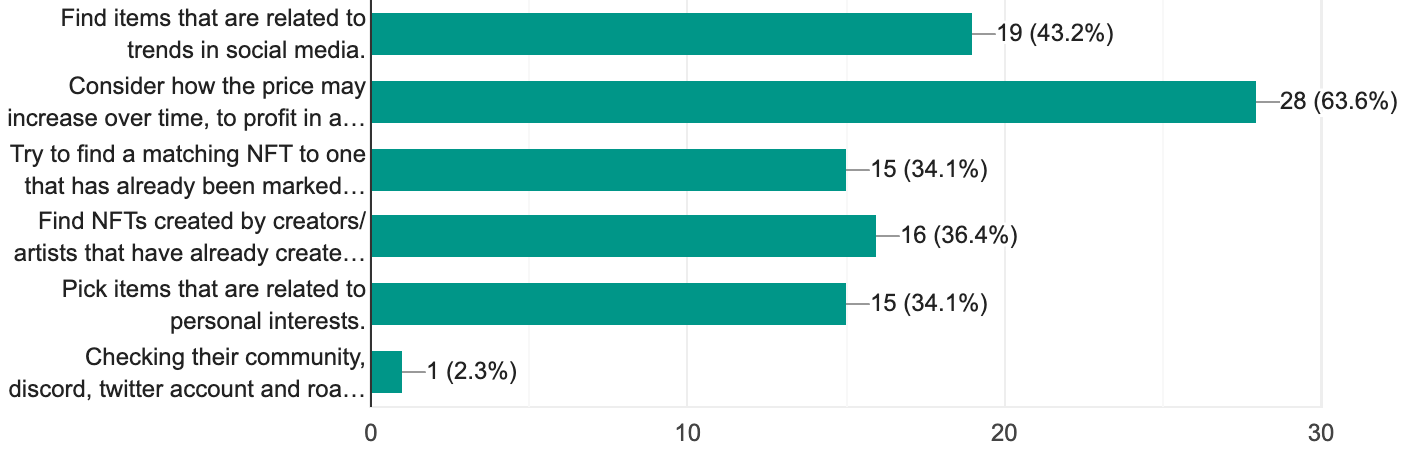
\includegraphics[width=\textwidth]{images/SRS/survey/survey-1.png}
}
\\
\multicolumn{2}{|l|}{
\parbox{\textwidth}{
A majority of the participants thought that considering the price increase over time would be the primary factor of consideration when purchasing an \gls{nft}, while the second most impact to be considered was trends in social media. Finding NFTs that have been created by creators/ artists who have created valuable \gls{nft}s in the past, an \gls{nft} that is similar to what is already highly valuable and picking items related to personal interests saw similar weightings when making purchase decisions.
}
}

% \multicolumn{2}{|l|}{
% \parbox{\textwidth}{
% \begin{wrapfigure}{l}{0.70\textwidth}
% 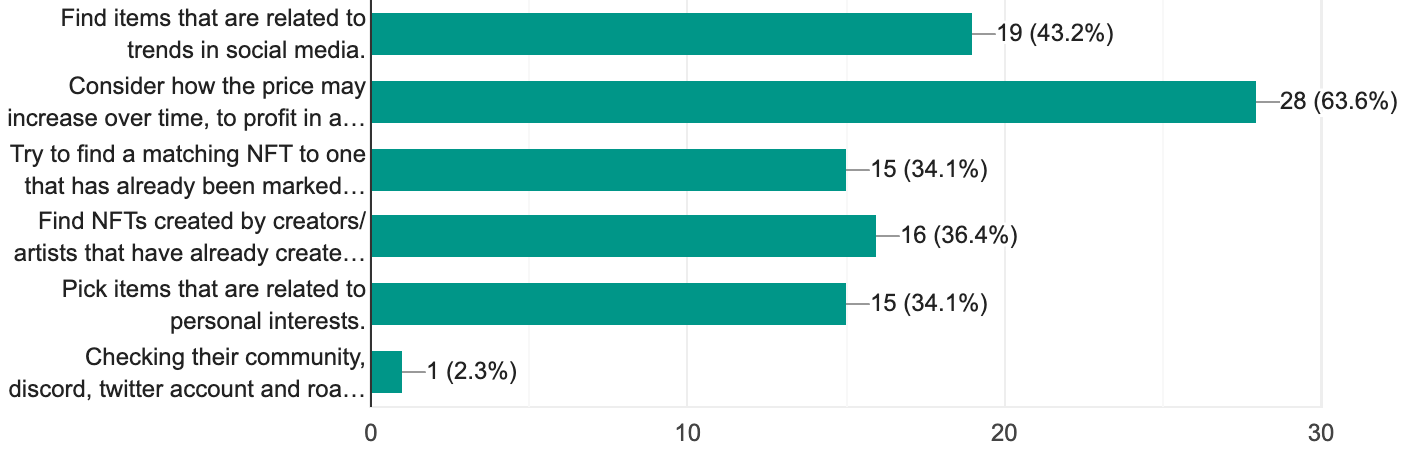
\includegraphics[width=0.70\textwidth]{images/SRS/survey/survey-1.png}
% \end{wrapfigure}

% A majority of the participants thought that considering the price increase over time would be the primary factor of consideration when purchasing an \gls{nft}, while the second most impact to be considered was trends in social media. Finding NFTs that have been created by creators/ artists who have created valuable \gls{nft}s in the past, an \gls{nft} that is similar to what is already highly valuable and picking items related to personal interests saw similar weightings when making purchase decisions.
% }
% }
\\
\hline
\textbf{Question} & \textbf{Who do you think will be benefited from using this system?} \\
\hline
\textbf{Aim of question} & To identify the beneficiaries of the proposed system. \\
\hline
\multicolumn{2}{|l|}{\textbf{Findings \& Conclusions}} \\

\multicolumn{2}{|l|}{
\parbox{\textwidth}{
\begin{wrapfigure}{l}{0.5\textwidth}
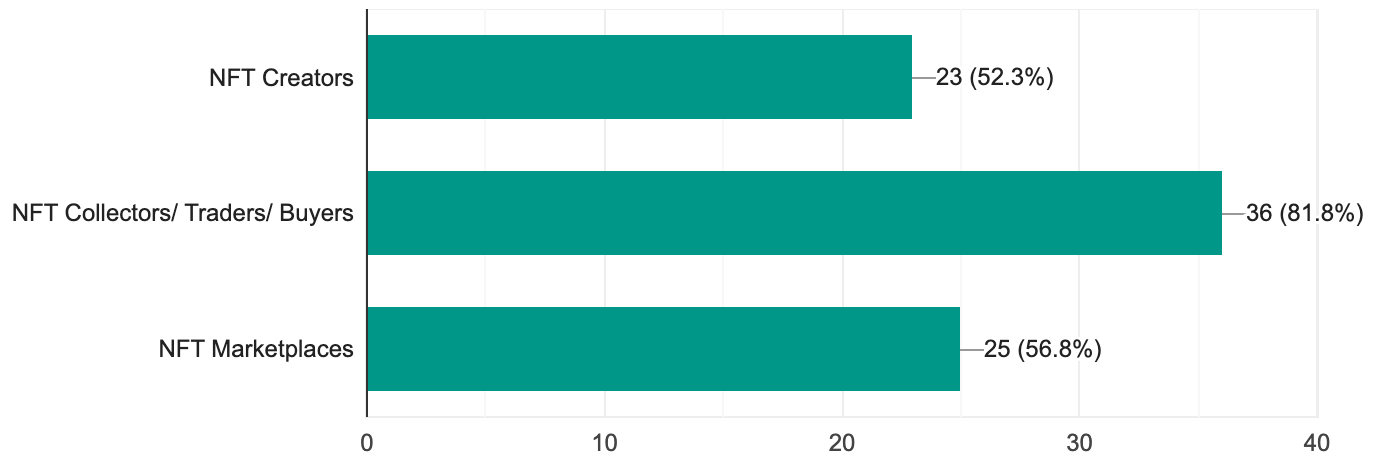
\includegraphics[width=0.5\textwidth]{images/SRS/survey/survey-2.png}
\end{wrapfigure}

While more than 50\% of participants aggreed that the proposed system would benefit the suggested beneficiaries, 81.8\% thought that \gls{nft} collectors/ traders/ buyers would benefit. Since, they are the ultimate target users, it's satisfying to see such positive responses.
}
}
\\
\hline
\textbf{Question} & \textbf{Do you think that this system would benefit people who have no expertise in Blockchain/ NFTs as well as people who have a decent amount of expertise in Blockchain/ NFTs?} \\
\hline
\textbf{Aim of question} & To identify how valuable the system would be to people of all levels of expertise in Blockchain/ NFTs \\
\hline
\multicolumn{2}{|l|}{\textbf{Findings \& Conclusion}} \\

\multicolumn{2}{|l|}{
\parbox{\textwidth}{
\begin{wrapfigure}{l}{0.53\textwidth}
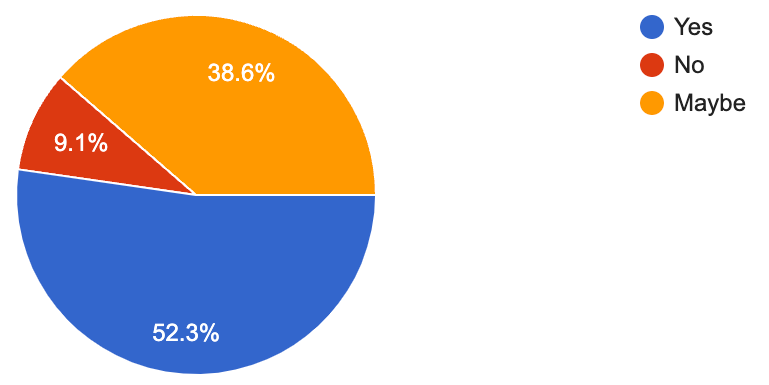
\includegraphics[width=0.46\textwidth]{images/SRS/survey/survey-3.png}
\end{wrapfigure}

With majority of the responses suggesting that people of all levels of expertise in Blockchain/ NFTs would benefit from the system depicts that the proposed system would be beneficial for above-average users as well.

}
}
\\
% \pagebreak
\hline
\textbf{Question} & \textbf{How much do you think that a Recommendations System would benefit you, if you ever plan on purchasing an NFT?} \\
\hline
\textbf{Aim of question} & To identify if the respondents think that the system would benefit them. \\
\hline
\multicolumn{2}{|l|}{\textbf{Findings \& Conclusion}} \\

\multicolumn{2}{|l|}{
\parbox{\textwidth}{
\begin{wrapfigure}{l}{0.6\textwidth}
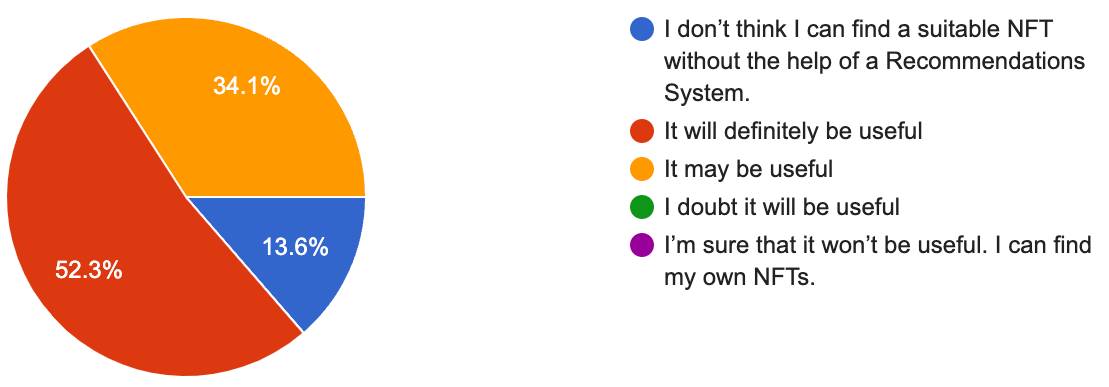
\includegraphics[width=0.6\textwidth]{images/SRS/survey/survey-4.png}
\end{wrapfigure}

52.3\% of users thought that a Recommendations System would definitely be useful to them if they plan on purchasing an \gls{nft}, while 34.1\% thought that it may be useful. Meanwhile, 13.6\% of users thought that they don't think that they could find a suitable \gls{nft} without the help of a Recommendations System. 100\% of the results were aligned towards seeing a possible benefit of the proposed system.
}
}
\\
\hline
\textbf{Question} & \textbf{How much would you expect a Recommendations System that considers social media trends to be beneficial for businesses to integrate into their online platforms?} \\
\hline
\textbf{Aim of question} & To identify the importance of the technological contribution in the project \\
\hline
\multicolumn{2}{|l|}{\textbf{Findings \& Conclusion}} \\

\multicolumn{2}{|l|}{
\parbox{\textwidth}{
\begin{wrapfigure}{l}{0.48\textwidth}
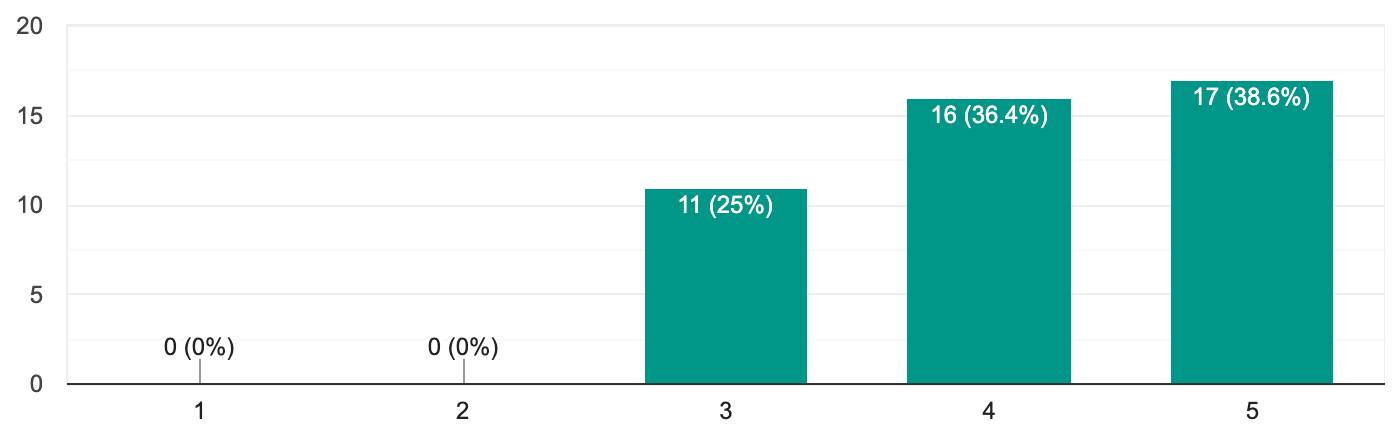
\includegraphics[width=0.48\textwidth]{images/SRS/survey/survey-5.png}
\end{wrapfigure}

The results from this question suggests that the technological contribution that has been highlighted in this project, which addresses an advancement of development of Recommendation Systems is expected to be extremely beneficial for business applications.
}
}
\\
\hline
\textbf{Question} & \textbf{Do you think that a user would benefit more if one platform provides recommendations that differ from another platform with the same dataset?} \\
\hline
\textbf{Aim of question} & To identify if the proposed Recommendations System will benefit from implementing a Reinforcement Learning technique or a variable bias to adapt and suite different platforms. \\
\hline
\multicolumn{2}{|l|}{\textbf{Findings \& Conclusion}} \\

\multicolumn{2}{|l|}{
\parbox{\textwidth}{
\begin{wrapfigure}{l}{0.5\textwidth}
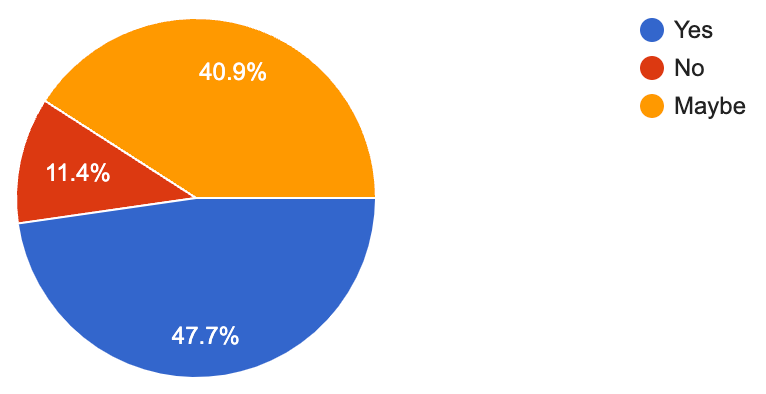
\includegraphics[width=0.5\textwidth]{images/SRS/survey/survey-6.png}
\end{wrapfigure}

A majority of participants thought that having varied recommendations in different platforms, using the same recommendations algorithm. This leads to the requirement of implementing a variable bias towards the factors considered for recommendations or implementing a reinforcement learning technique, for the model to adjust based on user-inputs. Having a pre-configurable bias will also allow to achieve this, but the results from recommendations may not be optimum.
}
}
\\
\hline
\textbf{Question} & \textbf{What functionalities would you like to have in a Trading Recommendations System for Non-fungible Tokens?} \\
\hline
\textbf{Aim of question} & To identify the non-function requirements of the system, that would make the system as user-friendly as possible \\
\hline
\multicolumn{2}{|l|}{\textbf{Findings \& Conclusion}} \\

\multicolumn{2}{|l|}{
\parbox{\textwidth}{
Most responses form the participants revolved around considering price-predictions when making recommendations. There were also suggestions to integrate trending crypto news to the system. Suggesting potential \gls{nft}s that suit a person's personal interests were also suggested to be integrated.
}} \\ 
\hline
% \textbf{Question} & \textbf{How knowledgeable are you about Blockchain technology? How knowledgeable are you about NFTs? Which of the following roles describes your relevance of expertise to this project?} \\
% \hline
% \textbf{Aim of question} & To identify the background of the target audience and identify which of their responses will be more valuable for the domain contribution and technological contribution.  \\
% \hline
% \multicolumn{2}{|l|}{\textbf{Findings}} \\
% \hline
% \multicolumn{2}{|l|}{} \\ 
% \hline
\end{longtable}


\subsection{Prototyping}
% \vspace{-4mm}       % remove line spacing after
% \begin{longtable}{|p{0.96\linewidth}|}
% \caption{Findings through Prototyping}\\
% \hline
% \textbf{Findings} \\
% \hline
Through iterative prototyping, there were many requirements \& challengers that emerged. Firstly, there was no dataset. The data had to be pulled from an open \gls{api} and filtered. The main challenge that was met here was the overwhelming amount of data that was received related to each \gls{nft} and rate limits of the \gls{api}. The data received had to be filtered quite a lot and the most usable data points possible to be used for recommendations had to be identified \& extracted. Not all \gls{nft}s contained usable content-information. This had to be addressed with normalizing several fields and finding alternatives to map items using other available data.
\\
The integration of social trends data brought in a new valid perspective that could be used for recommendations.
% \\
% \hline
% \end{longtable}

% \pagebreak
\section{Summary of Findings}

\vspace{-4mm}
\begin{longtable}{|l|p{0.72\linewidth}|c|l|l|l|}
\caption{Summary of Findings}\\ 
\hline
\textbf{Id} & \textbf{Finding} & \begin{turn}{-90} \parbox{5.2em}{\setstretch{0.8}{\textbf{Literature Review}}} \end{turn} & \begin{turn}{-90}\textbf{Interviews}\end{turn} & \begin{turn}{-90}\textbf{Survey}\end{turn} & \begin{turn}{-90}\textbf{Prototyping}\end{turn}  \endfirsthead 
\hline
1 & The proposed system would benefit experienced \& inexperienced users searching for \gls{nft}s as well as \gls{nft} creators, traders \& market places &  \checkmark  & \checkmark & \checkmark  &    \\ 
\hline
2 & The limits of Recommendation Systems can be pushed without the use of Deep learning, by the application of various hybrid ensemble models & \checkmark & \checkmark  &  &  \\
\hline
3 & The integration of social media trends would be beneficial to improve recommendations produced by a Recommendations System & \checkmark & \checkmark & \checkmark & \checkmark  \\
\hline
4 & The identified research gap would contribute to both the Blockchain-\gls{nft} domain as well as the advancement of Recommendations Systems \& \gls{ml} & \checkmark & \checkmark & \checkmark &  \\
\hline
5 & Building custom use-case specific algorithms for the Recommendations System is prefered over the use of pre-built models from a business application perspective &  & \checkmark &  &   \\
\hline
6 & Having a method of price-prediction \& using the prediction data to make decisions on recommendations would benefit users &  & \checkmark & \checkmark &   \\
\hline
7 & Using data-clustering techniques to identify contract-recognition \& data tags are expected by advanced-users &  & \checkmark &  &   \\
\hline
8 & Personalized recommendations could be achieved by the use of information extracted from the Blockchain with related to a user's public key. Past purchases of \gls{nft}s made by users can be considered. & \checkmark & \checkmark &  &   \\
\hline
9 & It would be good to have a user-interface that allows the user to choose the bias/ his primary concerns when expecting a recommendation, to provide the perfect recommendation for each user. &  & \checkmark &  &   \\
\hline
9 & Having a adaptable, variable Recommendations Model that allows different platforms to have varied recommendations is preferred. &  & \checkmark & \checkmark &   \\
\hline
10 & Having a sufficient set of well-cleaned \& pre-processed data would be vital for the performance of the system & \checkmark & \checkmark &  & \checkmark \\
\hline
11 & Opinions of well-known influencers could have a bigger impact on the decision-making process of a majority of users. &  & \checkmark &  &  \\
\hline
\end{longtable}


\section{Context Diagram}
Prior to development, the system's boundaries and interactions should be determined. The system's context is depicted in the diagram below.

% context diagram draw.io: https://app.diagrams.net/#G1L3yGzZMl_wCd4_qT4tBV2uCwffqsAuol

\begin{figure}[h!]
\centering
\setlength{\fboxsep}{10pt}%
\setlength{\fboxrule}{0.5pt}%
\fbox{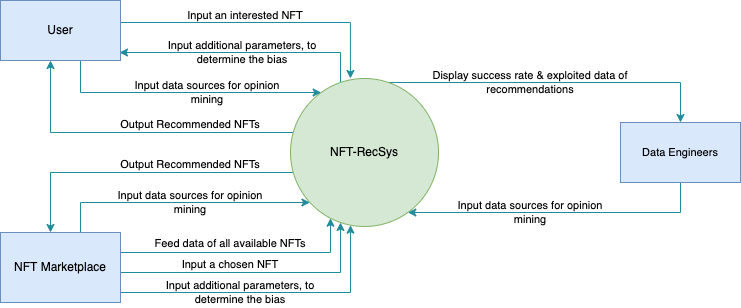
\includegraphics[width=0.95\textwidth]{images/SRS/context-diagram.png}}
\caption{Context Diagram \textit{(self-composed)}}
\label{fig:context-diagram}
\end{figure}

\pagebreak
\section{Use Case Diagram}

\begin{figure}[h!]
\centering
\frame{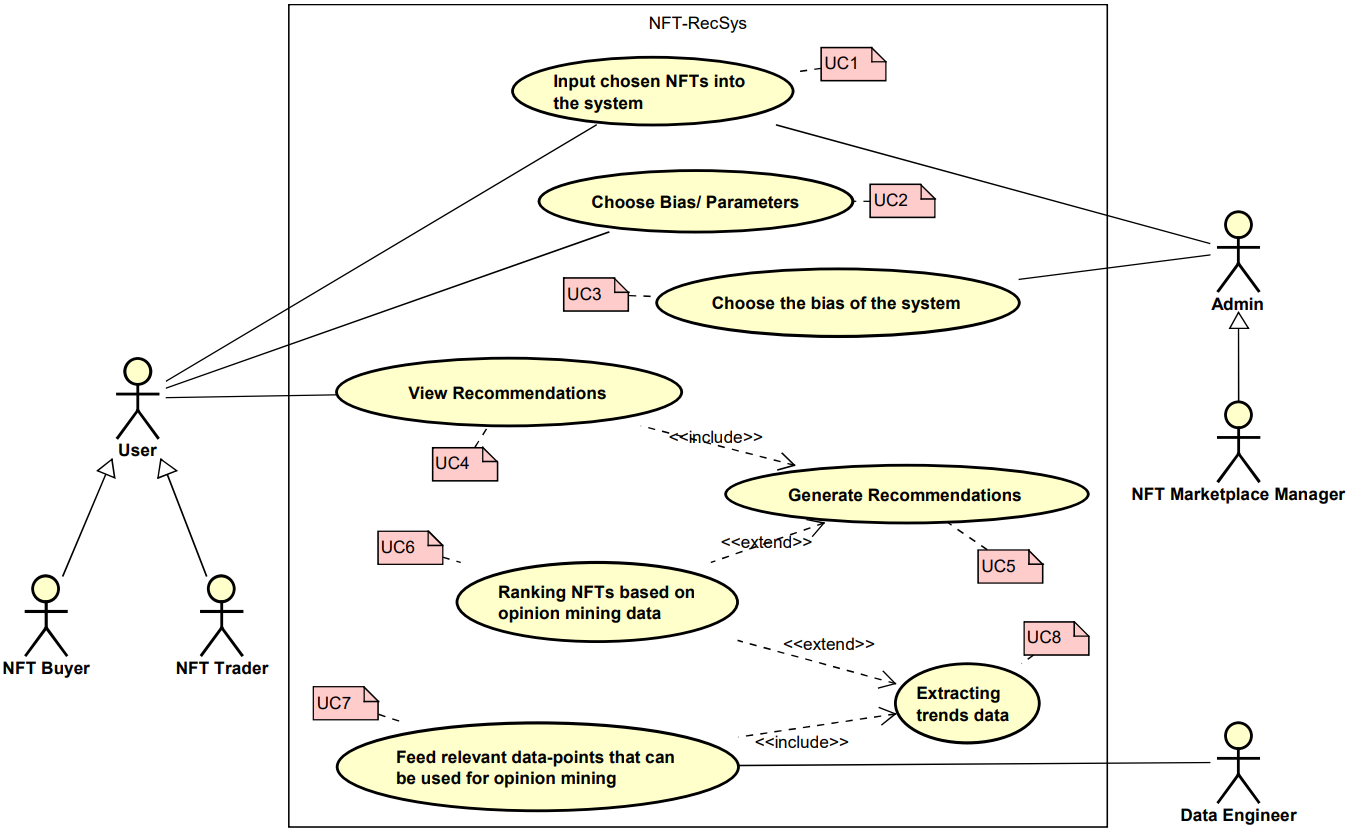
\includegraphics[width=\textwidth]{images/SRS/use-case-diagram.png}}
\caption{Use Case Diagram \textit{(self-composed)}}
\label{fig:use-case-diagram}
\end{figure}


\section{Use Case Descriptions}

\vspace{-4mm}
\begin{longtable}{|p{0.23\linewidth}|p{0.73\linewidth}|}
\caption{Use case description UC:04}\\ 
\hline
Use Case & View Recommendations \endfirsthead 
\hline
Id & UC:04 \\ 
\hline
Description & Display the most relevant \gls{nft} Recommendations based on the user's selection \& available data in the system. \\ 
\hline
Primary Actor & User \\ 
\hline
Supporting Actors (if any) & none \\ 
\hline
Stakeholders and Interests (if any) & Admins, \gls{nft} Traders, \gls{nft} creator \\ 
\hline
Pre-‐Conditions & The \gls{nft} data and trends data have to have been pre-processed. The recommendations have to have been generated. \\ 
\hline
Post Conditions & Success end condition: The user is presented with recommended \gls{nft}s. \\ 
\hline
Trigger & A user wishes to find similar \gls{nft}Ts to those that are currently being viewed or to explore possible interests based on past views. \\ 
\hline
Main Success Scenario & 
\vspace{-7mm}       % remove line spacing before itemize
\begin{itemize}[leftmargin=*]
\item User chooses the option to view recommendations.
\item System recognizes the user's preferred bias for recommendations.
\item System filters out and diversifies recommendations based on the user-bias and general bias that has been set in the system.
\item System displays the recommended NFTs. 
\end{itemize}
\vspace{-7mm}       % remove line spacing after itemize
\\ 
\hline
Variations & A user can be presented with recommended NFTs based on past interests shown and views in a feed similar to a social network/ e-commerce store. \\
\hline
\end{longtable}

\vspace{-4mm}
\begin{longtable}{|p{0.23\linewidth}|p{0.73\linewidth}|}
\caption{Use case description UC:07}\\ 
\hline
Use Case & Ranking \gls{nft}s based on Opinion mining data \endfirsthead 
\hline
Id & UC:07 \\ 
\hline
Description & Rank \gls{nft}s for recommendations based on gathered social media trends data, opinion mining data \& content in \gls{nft}s. \\ 
\hline
Primary Actor & none \\ 
\hline
Supporting Actors (if any) & Admins, Users \\ 
\hline
Stakeholders and Interests (if any) & \gls{nft} Collectors, \gls{nft} Traders, \gls{nft} creator \\ 
\hline
Pre-‐Conditions & New data-points have been added by an admin or a user and the trends have been extracted. \\ 
\hline
Post Conditions & Success end condition: Rank \gls{nft}s \\ 
\hline
Trigger & An admin or a user wishes to find \gls{nft}s that have content related to what's trending on the internet at the current moment in time. \\ 
\hline
Main Success Scenario & 
\vspace{-7mm}       % remove line spacing before itemize
\begin{itemize}[leftmargin=*]
    % \item System pre processes new opinion mining data to produce extracted trends data.
    \item System matches data of each \gls{nft} in the current data-set with extracted trends data.
    \item System calculates a score for each \gls{nft} based on the matches \& impact of the identified trends.
    \item System re-ranks \gls{nft}s based on the calculated scores.
\end{itemize}
\vspace{-7mm}       % remove line spacing after itemize
\\ 
\hline
Variations & When recommendations are produced using other methods apart from trends, the data ranking scores generated here can be used to re-rank the recommendations when presenting to a user. \\
\hline
\end{longtable}


\section{Requirements}

\subsection{Functional Requirements}
The MoSCoW technique was used to determine the priority levels of system needs based on their importance.

\begin{longtable}{|l|p{0.77\linewidth}|}
\caption{Levels of priority according to the "MoSCoW" technique.}\\ 
\hline
\textbf{Priority Level} & \textbf{Description}                                                                                                    \endfirsthead 
\hline
Must have (M)           & This level's requirement is a prototype's core functional requirement, and it must be implemented.                      \\ 
\hline
Should have (S)         & Important requirements aren't absolutely necessary for the expected prototype to work, but they do add a lot of value.  \\ 
\hline
Could have (C)          & Desirable requirements that are optional and aren't deemed essential critical to the project's scope.                   \\ 
\hline
Will not have (W)       & The requirements that the system may not have and that are not considered a top priority at this time.                  \\
\hline
\end{longtable}


\begin{longtable}{|l|p{0.71\linewidth}|c|l|}
\caption{Functional requirements}\\ 
\hline
\begin{tabular}[c]{@{}l@{}}\textbf{FR}\\\textbf{ID}\end{tabular}
& \textbf{Requirement} & \begin{tabular}[c]{@{}c@{}}\textbf{Priority}\\\textbf{Level}\end{tabular} & 
\begin{tabular}[c]{@{}c@{}}\textbf{Use}\\\textbf{Case}\end{tabular}
\endfirsthead 
\hline
FR1 & Users must be able to add a chosen NFT to be considered as the reference point to generating recommendations. & M & UC1 \\ 
\hline
FR2 & Admins should be able to add a collection of NFT to be used as recommendations. & S & UC1 \\ 
\hline
FR3 & The system could be able to fetch relevant data of the NFT using an entered contract address \& token Id. & C & UC1 \\ 
\hline
FR4 & Users must be able to set/ adjust the bias and parameters to be used by the Recommendations System using parametric selections prior to generating recommendations. & M & UC2 \\ 
\hline
FR5 & Admins should be able to choose the bias of the Recommendations System. & S & UC3 \\ 
\hline
FR6 & Users must be able to view recommendations with the click of a button. & M & UC4 \\
\hline
FR7 & The prototype could have an option to receive user feedback regarding the satisfaction level of the generated recommendations by the system. & C & UC4 \\
\hline
FR8 & The system could show the reasons for recommending each item to users. & C & UC4 \\ 
\hline
FR9 & The system should generate recommendations based on what the user expects to view & S & UC5 \\ 
% \hline
% FR9 & The system should generate price predictions and consider the results for recommendations. & S & UC5 \\ 
\hline
FR10 & Opinion mining trends data must be used to generate \gls{nft} recommendations. & M & UC8\\
% \hline
% FR11 & A user could be allowed to feed data-points such as interested public figures, websites to use as opinion mining data for recommendations. & C & UC8 \\ 
\hline
FR11 & Admins could be allowed to feed data-points such as various social networks, interested public figures, websites to use as opinion mining data for recommendations. & C & UC7 \\
\hline
FR12 & User-input could be used as a reinforcement learning bias for the Recommendations Model. & C & NA  \\
\hline
FR13 & The system will not act as a decentralized system. & W & NA \\
\hline
% FR15 search NFTs by tags?
\end{longtable}

% \pagebreak
\subsection{Non-functional Requirements}
\vspace{-4mm}
\begin{longtable}{|l|l|p{0.5\linewidth}|l|}
\caption{Non-functional requirements}\\ 
\hline
\textbf{NFR ID} & \textbf{Requirement} & \textbf{Description} & \textbf{Priority Level} \endfirsthead 
\hline
1 & Performance & Although recommendations should be provided upon user-input; the recommendations matrix \& opinion-mining data can be pre-processed and stored in-memory to be used. Real-time processing isn't essential. & Desirable \\ 
\hline
2 & Quality of Output & The quality of the output should be of the highest possible level, utilizing all the available data. & Important \\ 
\hline
3 & Security & The application should prevent any attackers from manipulating results and extracting user-inputs. Security could be assured by means of testing. & Desirable \\ 
\hline
4 & Usability & Since the purpose of the system is to automate and make it easy for the user to explore NFTs, the usability of the system must be easy for users of all levels of expertise. & Important \\ 
\hline
5 & Scalability & The prototype may open up for testing for many users. Considering the hype around \gls{nft}s and the interest in the project, the system may have to support many concurrent user-requests. & Desirable \\
\hline
\end{longtable}


\section{Chapter Summary}
In this chapter, a Rich Picture Diagram was drawn to illustrate how the system connects with the society to understand the stakeholders of the system. Saunder's Onion model was used to represent the stakeholders with the flow of influence of each stakeholder. Requirement gathering techniques were utilized to gather all the required data and opinions of possible stakeholders of the system. Lastly, the system's use cases, functional, and non-functional requirements were specified based on the insights derived from the requirement elicitation techniques.